\documentclass[12pt, a4paper]{article}

\usepackage[hmargin=2.5cm, vmargin=2cm]{geometry}
\usepackage{amsthm, amssymb, mathtools, yhmath, graphicx}
\usepackage{fontspec, type1cm, titlesec, titling, fancyhdr, tabularx}
\usepackage{color, unicode-math, float, hhline}

\usepackage[CheckSingle, CJKmath]{xeCJK}
\usepackage{CJKulem}
\usepackage{enumitem}
\setenumerate{itemsep=0pt}
\usepackage{tikz}
\usepackage{circuitikz}
\usepackage{hyperref}
\usepackage{minted}
\usepackage{lipsum}
\BeforeBeginEnvironment{minted}{\vspace*{-5mm}}
\AfterEndEnvironment{minted}{\vspace*{-5mm}}
\usetikzlibrary{matrix}

\usepackage[backend=biber, style=verbose]{biblatex}
\bibliography{lab1.bib} 

\setmainfont{Linux Libertine O}
\setmonofont{Source Code Pro}
\setCJKmainfont{Source Han Sans TC}

\def\codesize{\fontsize{10}{15}\selectfont}
\def\normalsize{\fontsize{12}{18}\selectfont}
\def\large{\fontsize{14}{21}\selectfont}
\def\Large{\fontsize{16}{24}\selectfont}
\def\LARGE{\fontsize{18}{27}\selectfont}
\def\huge{\fontsize{20}{30}\selectfont}

%\titleformat{\section}{\bf\Large}{\arabic{section}}{24pt}{}
%\titleformat{\subsection}{\large}{\arabic{subsection}.}{12pt}{}
%\titlespacing*{\subsection}{0pt}{0pt}{1.5ex}

\parindent=0pt
\parskip=1em

\DeclarePairedDelimiter{\abs}{\lvert}{\rvert}
\DeclarePairedDelimiter{\norm}{\lVert}{\rVert}
\DeclarePairedDelimiter{\inpd}{\langle}{\rangle}
\DeclarePairedDelimiter{\ceil}{\lceil}{\rceil}
\DeclarePairedDelimiter{\floor}{\lfloor}{\rfloor}

\setminted[sv]{
  linenos=true, frame=lines, framesep=2mm,
  fontsize=\codesize
}
\setminted[bash]{
  linenos=true, frame=lines, framesep=2mm,
  fontsize=\codesize
}

\newcommand{\img}{\mathsf{i}}
\newcommand{\ex}{\mathsf{e}}
\newcommand{\dD}{\mathrm{d}}
\newcommand{\dI}{\,\mathrm{d}}

\title{數位電路實驗 Lab-1 教學手冊 -- 點名器}
\author{Team \#2}
\begin{document}
\maketitle

\section{概述}
有鑑於網路上 Quartus 關於 Linux 系統以及 Command line tools 的資源較少,這邊希望能將
這些資訊整理一下,或許可以幫助一些有需要的人。

因此這篇教學文件會著重在
\begin{enumerate}
  \item Linux 上的環境架設。
  \item Command line tool 的使用。
\end{enumerate}

\section{安裝 Quartus}
Linux 安裝 Quartus 直接在官方網站\footcite{QuartusDL}下載即可。 \\

但注意的事 Quartus 最新版在某些 Linux Distro. 下編譯會非常慢甚至卡住。
似乎是 Quartus 的 bug,在編譯的時候切斷網路可以部份解決問題\footcite{QuartusBugHack}(但在最後一
步需要連上網路驗證 License 才會有輸出檔)。目前已知在 Ubuntu, Mint 下似乎不會有問題。

\section{Command line tool}
Quartus 其實提供了算是完整的 Command line tools,許多功能不用開起 Quartus GUI 也
可以完成,這對於習慣在 Command line 下工作或是使用如 Vim 編輯器的人無疑是一大
福音!

\subsection{Quartus 相關}
可以參考官方的說明文件\footcite{QuartusCmdRef}。\\
{\bf 建議是第一次用 Quartus GUI 建立 Projects,並且用內建的
Programmer 燒過一次 \texttt{.sof} 檔,之後再用 Command line tools。} \\
以下是一個參考用的 \texttt{Makefile}。
\begin{minted}[
  linenos=true, frame=lines, framesep=2mm, fontsize=\codesize
]{makefile}
QUARTUS_SH = quartus_sh
QUARTUS_PGM = quartus_pgm
FLAGS = --flow compile
PROJECT = lab1
OUTPUT = output_files
CABLE = USB-Blaster

.PHONY: all clean flash

all: sof

sof:
  $(QUARTUS_SH) $(FLAGS) $(PROJECT)

flash:
  $(QUARTUS_PGM) -c $(CABLE) chain.cdf

clean:
  rm $(OUTPUT)/$(PROJECT).sof$
\end{minted}
建議將 Smart Compile 開起,可節省不少時間。 \\
如果要加入新檔案,可能要自行修改 \texttt{.qsf} 加入類似以下的指令
\begin{minted}[
  linenos=true, frame=lines, framesep=2mm, fontsize=\codesize
]{sh}
set_global_assignment -name SYSTEMVERILOG_FILE xxx.sv
\end{minted}
\subsection{Qsys 相關}
就用 Quartus GUI 做吧… 其實他的介面還算不錯!
\subsection{Nios II 相關}
{\bf 與 1 類似,建議是第一次用 Quartus 開起 Ellipse 建立 Project,
並且燒上 Cyclone。 } 之後 Ellipse 會自動幫你建好一個 \texttt{Makefile},
直接使用即可。

\section{實做細節}
這個實驗其實主要就是要完成一個 State Machine。
\begin{figure}[H]
  \centering
  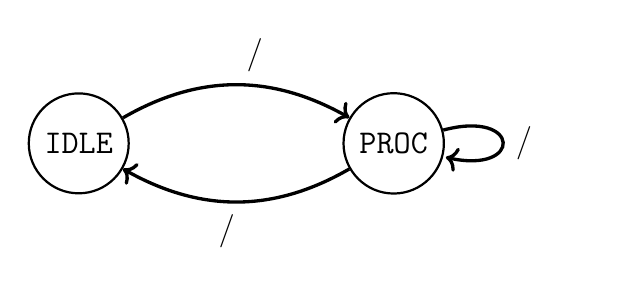
\begin{tikzpicture}
    \node[draw, circle, thick] (v1) at (0, 0) {\texttt{IDLE}};
    \node[draw, circle, thick] (v2) at (4, 0) {\texttt{PROC}};
    \path[very thick, ->, bend left] (v1) edge node[midway, above]{按下按鈕/} (v2) ;
    \path[very thick, ->] (v2) edge[loop right] node[midway, right]{/變換數字、漸慢} (v2) ;
    \path[very thick, ->] (v2) edge[bend left] node[midway, below]{/結束} (v1) ;
  \end{tikzpicture}
\end{figure}
可用以下電路來實做:
\begin{figure}[H]
  \centering
  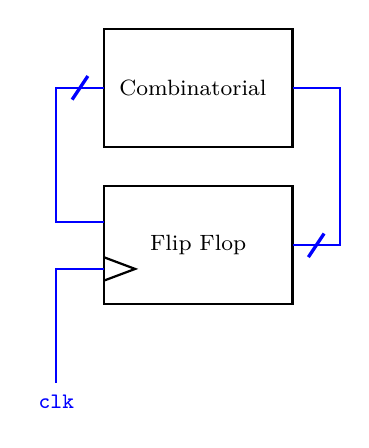
\begin{tikzpicture}
    \draw[thick] (0, 0) rectangle (2.4, 1.5)node[pos=.5]{\footnotesize Flip Flop};
    \draw[thick] (0, 2) rectangle (2.4, 3.5)node[pos=.5, text width=2cm]{\footnotesize Combinatorial};
    \draw[thick, blue] (2.4, 0.75) -| (3, 2.75) -- (2.4, 2.75);
    \draw[very thick, blue] (2.8, 0.9) -- (2.6, 0.6);
    \draw[thick, blue] (0, 2.75) -| (-0.6, 1.05) -- (0, 1.05);
    \draw[very thick, blue] (-0.2, 2.9) -- (-0.4, 2.6);
    \draw[thick] (0, 0.3) -- (0.4, 0.45) -- (0, 0.6);
    \draw[thick, blue] (0, 0.45) -- (-0.6, 0.45) -- (-0.6, -1) node[below]{\footnotesize \texttt{clk}};
  \end{tikzpicture}
\end{figure}

似乎有看過兩種寫法:
\begin{minted}{sv}
wire w1 = ...;
wire w2 = ...;
logic m1, m2;
other declaration...

always_ff @(posedge clk or posedge rst) begin
  if (rst) begin
    preform reset ...
  end else begin
    if (some condition) begin
      m1 <= w1;
      ...
    end
    if (some other condition) begin
      m2 <= w2;
      ...
    end
    ...
  end
end
\end{minted}
這種寫法在 \mintinline{sv}{always_ff} 裡做判斷,比較輕便好寫,但程式大了、
邏輯複雜時似乎不好維護。

另一種寫法是
\begin{minted}{sv}
logic m1_r, m1_w;
logic m2_r, m2_w;
other declaration...

always_comb begin
  m1_w = ...
  m2_w = ...
  if (some condition) begin
    m1_w = ...
    m2_w = ...
  end else begin
    m1_w = ...
    m2_w = ...
  end
end

always_ff @(posedge clk or posedge rst) begin
  if (rst) begin
    preform reset ...
  end else begin
    m1_r <= m1_w;
    m2_r <= m2_w;
    ...
  end
end
\end{minted}
這種寫法將 Combinatorial 和 Sequential 分開,似乎比較乾淨。不
過似乎比較冗長,而且 \texttt{\_r}, \texttt{\_w} 很容易眼花看錯…

State 可以用 \mintinline{sv}{case} 來處理,如果是使用 SystemVerilog
可以搭配 \mintinline{sv}{enum} 使用增加可讀性。
\begin{minted}{sv}
typedef enum {
  STATE1,
  STATE2,
  ...
} State_t

State_t state_r, state_w;

initial begin
  state_r = STATE1; // Initial state
  ...
end

always_comb begin
  state_w = state_r;
  case (state_r)
    STATE1: begin
      ...
      state_w = STATE2; // Next state
    end
    STATE2: begin
      ...
    end
  endcase
end

always_ff @(posedge clk or posedge rst) begin
  if (rst) begin
    state_r <= STATE1; // Initial State
    ...
  end else begin
    state_r <= state_w;
    ...
  end
end
\end{minted}

\section{Random Generator}
似乎使用一個 linear congruential generator 就可以有不錯的效果了。
Linear congruential generator 使用的公式為
\[ X_{n+1} = a X_n + b \pmod{M} \]
也就是下一個數字是前一個數字乘一個常數後加上一個常數在模 $M$ 。
{\bf 建議最後把 $X$ 的末幾個 Bit 捨棄掉,因為後面幾個 Bit 的
循環節很短。 } 比如說如果 $M$ 有 $32$ 位,而最後只需要 $8$ 位
的亂數,不要取 \texttt{X[7:0]} 而是取如 \texttt{X[23:16]} 。

而如果希望系統重設時亂數的結果可以不一樣(不要第一次的結果一定是
$a_1$,第二次的結果一定是 $a_2$ 等等),可以考慮讓產生的結果和
使用者按下的時間有關。一個可行的做法是每一個 clock 就 tick 
一次 random generator 而不是使用者每按一次才 tick 一次。

\section{Time Delay}
時間延遲可以透過計算 clock 數得到。假設要延遲 $t$ 秒,而系統的
clock 為 $c$ Hz,那麼就相當於 $ct$ 個 clock。 可以如下實做 
\clearpage
\begin{minted}{sv}
int counter;
localparam int TICKS_PER_DELAY = ...;

always_comb begin
  if (counter >= TICKS_PER_DELAY) begin
    // Delay ended.. continue next procedure
    ...
  end
end

always_ff @(posedge clk) begin
  if (counter reset) 
    counter <= 0;
  else 
    counter <= counter + 1;
end
\end{minted}

\end{document}

